\documentclass{article}
\usepackage[utf8]{inputenc}
\usepackage[usenames,dvipsnames]{xcolor}
\usepackage{pdfpages}	  % Insertion of PDF-pages

% Sideopsætning
\usepackage{geometry}                       % Håndtering af papirstørrelse og marginer
\geometry{a4paper, twoside}                 % Papirstørrelse
\geometry{top=2.5cm, bottom=2.5cm}		    % Øvre og nedre margin
\geometry{left=2.5cm, right=2.5cm}		    % Venstre og højre margin

% Tekstformatering
\setlength{\parindent}{0pt}				    % Indryk
\linespread{1.2}							% Linjeafstand
\usepackage[dvipsnames]{xcolor, colortbl}	% Farvekommandoer
\newcommand{\myparagraph}[1]{\paragraph{#1}\mbox{}\\} % Paragraph med newline efter

\begin{document}

\section{IsLeapYear Diagram}
\begin{center}
    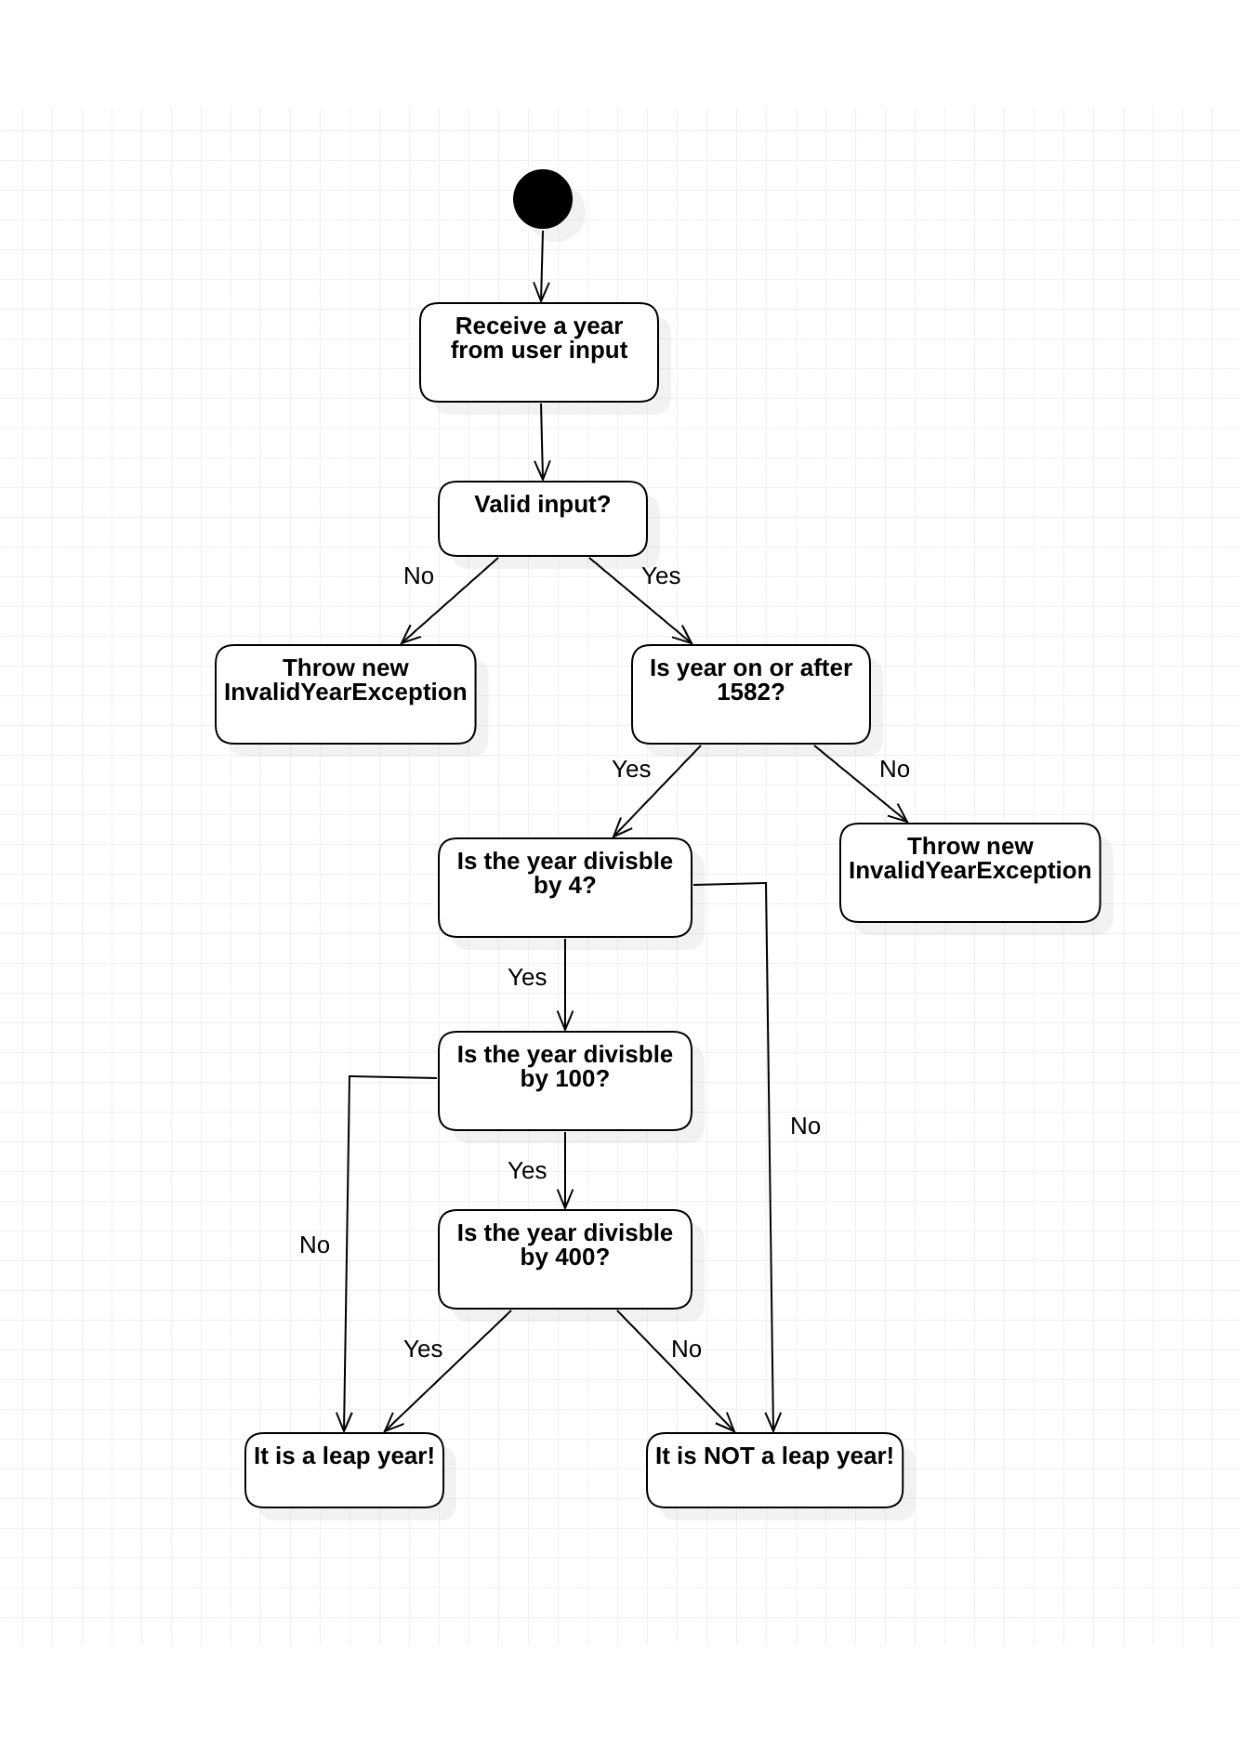
\includegraphics[width=\textwidth]{Diagrams/LeapYearUML.pdf}
    \label{FYMap}
\end{center}

\newpage

\section{IsLeapYear Diagram description}

This diagram shows how the program acts when executed. 
The user will first be asked for input, that is then validated in two steps. If the typed input cannot be converted to an integer, it will raise an exception, or else it will go to the next validation step. If it converts to am integer, but the year is earlier than 1582, it will also raise an exception. But if the input passes both of these steps, it will go on to the actual leap year determination.
First it will check if the year input is divisible by 4. If no, then it will go straight to the conclusion that the input is NOT a leap year.
If yes, then check if the year is divisible by 100. If it is not divisible by 100, then go to the conclusion that it is a leap year. If it is divisible by 100, the check if it is also divisible by 400. If it is divisible by 400, then it is a leap year. If it is not divisible by 400 also, then it is NOT a leap year.

\end{document}